\chapter{Prototipo sviluppato}
\label{chap:3}
Nel capitolo precedente sono state esaminate le differenze sostanziali tra un'approccio basato su Rust in combinazione con WebAssmebly e uno basato su Node.js.
In questo capitolo si presenterà il prototipo sviluppato con l'obiettivo di comprendere l'impatto di tali differenze in un'applicazione pratica.
\section{Descrizione dell'applicazione}
Il prototipo sviluppato è un applicazione dedicata all'elaborazione digitale di immagini, concepita per simulare un contesto realistico in cui le operazioni richiedono una considerevole quantità di elaborazioni da parte della CPU.
\\Dato il limitato tempo disponibile, non è stato possibile esplorare in dettaglio il vasto campo del \emph{digital image processing}. Pertanto, sono state impiegate librerie preesistenti in entrambi i linguaggi, evitando di immergersi eccessivamente nella programmazione di basso livello.
\\L'architettura dell'applicazione segue un modello client-server in entrambe le implementazioni.
Il cliente ha il compito di fornire i file da elaborare insieme alle relative specifiche sulle modifiche da apportare.
Il server eseguirà le modifiche richieste e restituirà al cliente il percorso della nuova immagine, pronta per il download.
\\Nel processo di selezione delle possibili modifiche da apportare, è stato essenziale individuare due librerie nei rispettivi linguaggi utilizzati.
Successivamente, per garantire uniformità nelle opzioni di modifica disponibili, sono state estratte le seguenti funzionalità comuni: 
\begin{itemize}
    \item ridimensionamento;
    \item rotazione di 90°;
    \item ribaltamento in orizzantale;
    \item conversione in bianco e nero;
    \item regolazione del contrasto;
    \item modifica della luminosità;
\end{itemize}
Tali operazioni sono state selezionate poiché rappresentano funzionalità frequentemente utilizzate anche da utenti comuni, oltre a caratterizzarsi per la loro eterogeneità. Alcune di queste coinvolgono esclusivamente la manipolazione dei pixel, come ad esempio la rotazione e il ribaltamento, mentre altre, come la conversione in scala di grigi o la modifica del contrasto/luminosità, comportano modifiche dirette ai pixel stessi.
\begin{figure}
    \centering
    \begin{minipage}{.5\textwidth}
      \centering
      
\includegraphics[width=.7\linewidth]{images/pre.jpeg}
    \end{minipage}%
    \begin{minipage}{.5\textwidth}
      \centering
      
\includegraphics[width=1\linewidth]{images/post.jpg}
    \end{minipage}
    \caption{Esempio di immagine a cui sono state apportate tutte le elaborazioni specificate.}
\end{figure}
\newpage
\section{Setup sperimentale}
\section{Metodologia}
\newpage
\section{Implementazione in Rust e Wasm/WASI}
Per quanto riguarda l'implementazione si è deciso di partire dal prototipo sviluppato in Rust poiché rappresentava l'aspetto più innovativo e richiedeva un considerevole impegno in termini di tempo.
\\Si è resa inoltre necessaria la ricerca di un framework che consentisse la creazione di un web server per la gestione delle richieste utente.
\\La scelta è ricaduta su actix-web, un web framework potente ed estremamente veloce per Rust.
\\Il client è costituito una semplice pagina html contenente un form per il caricamento delle immagini e due riquadri che mostrano l'immagine pre e post modifiche. Tale pagina eseguirà una richiesta AJAX al server, inviando il file da elaborare e le relative specifiche sulle modifiche. Successivamente il server restituirà il percorso della nuova immagine elaborata pronta per essere scaricata.
\begin{figure}
    \begin{center}
            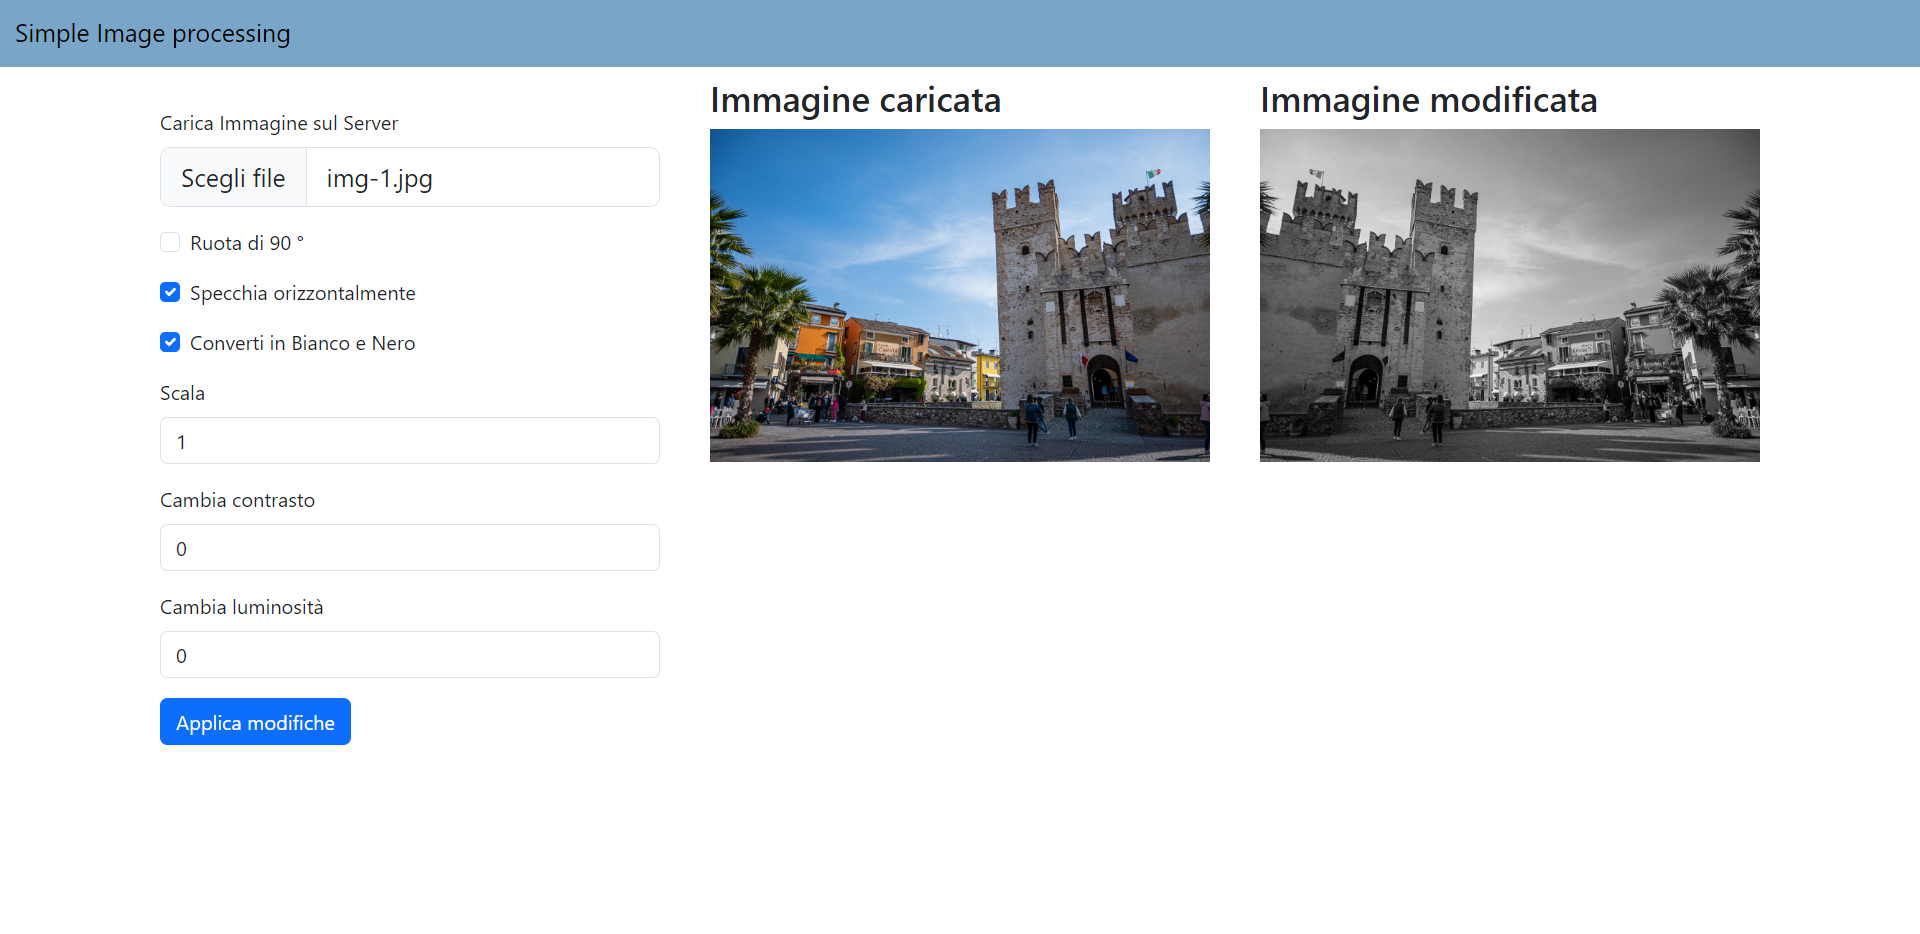
\includegraphics[width=1\columnwidth]{images/client.png}
    \end{center}
    \caption{View nel browser del client}
    \label{fig:client}
\end{figure}
\subsection{Actix-Web}
Lo studio del funzionamento di base del framework Actix-Web ha costituito un punto focale nella fase inziale dell'implementazione.
\\Tale framework si è dimostrato estremamente flessibile ed adatto per lo sviluppo del prototipo in questione.
Grazie all'impiego di \textbf{extractors}, di \textbf{handlers} e di altre funzionalità integrate, la gestione di richieste HTTP è risultata intuitiva e diretta.
\\La decisione di strutturare l'applicazione utilizzando diversi file è stata presa al fine di garantire un codice più ordinato e manutenibile.
Tra tutti i file, il principale è \textbf{main.rs}, che svolge un ruolo centrale nell'architettura complessiva.
\subsubsection{Configurazione server}
\begin{lstlisting}[language=rust, label=lst:RustWasi, caption={Porzione del file main.rs}, showstringspaces=false]
#[actix_rt::main]
async fn main() -> std::io::Result<()> {
    HttpServer::new(move || {
        App::new()
            .route("/", web::get().to(server::handlers::index))
            .route("/upload", web::post().to(server::handlers::upload))
            .service(fs::Files::new("/script", "./src/static/"))
            .service(fs::Files::new("/img", "./img/"))
            .app_data(state.clone())
    })
    .bind("127.0.0.1:8080")?
    .run()
    .await
}
\end{lstlisting}
Nel frammento di codice fornito, viene presentata la creazione di un HttpServer e un'istanza di App tramite il framework Actix-Web.
In Actix-Web, ogni server è costruito attorno a un'istanza di App, che consente di configurare le "regole di routing" per risorse di vario tipo, registrare servizi HTTP e gestire stato di livello applicazione.
\textbf{è presente lo state!!!!! cosa fare???}
\\Nel caso specifico, vengono configurate due regole di routing:
\begin{itemize}
    \item La prima regola gestisce le richieste dirette alla \textbf{home} del sito: in questo caso verrà semplicemente restituita la pagina index.html presente nella directory "static".
    \item La seconda regola gestisce richieste all'endpoint \textbf{upload}, per le quali è necessario ricevere un'immagine e le relative modifiche da apportare all'interno del modulo WebAssembly. Successivamente, verrà restituito il percorso della nuova immagine elaborata.
\end{itemize}
Si sottolinea che entrambe le regole di routing mappano le richieste a funzioni presenti all'interno del file \textbf{handlers.rs} nel modulo server.
\\Successivamente sono stati registrati due servizi HTTP  per garantire l'accesso a risorse statiche: script Javascript e immagini elaborate dall'applicazione.
\\Infine, dopo aver configurato il metodo di dispatching delle richieste ed aver messo a disposizione le risorse necessarie ai client, si è passati alla scrittura del codice nel file \textbf{handlers.rs}. Tale file, come suggerito dal nome, contiene gli handler delle richieste HTTP, con la conseguente esecuzione di codice WebAssmebly per richieste di modifica di immagini.

\begin{lstlisting}[language=Rust,caption={Operazioni principali presenti nel file handlers.rs}, showstringspaces=false]
#[derive(MultipartForm)]
pub struct ImageUpload {
    image: TempFile,
    scala: Text<f32>,
    contrasto: Text<f32>,
    luminosita: Text<i32>,
    ruota: Text<bool>,
    specchia: Text<bool>,
    bw: Text<bool>
}
#[derive(Serialize, Deserialize)]
pub struct Editings{
    scala: f32,
    ...
}
pub async fn index() -> HttpResponse {
    HttpResponse::Ok().content_type("text/html")
        .body(include_str!("../static/index.html"))
}

pub async fn upload(form: MultipartForm<ImageUpload>) -> HttpResponse {
    let time = SystemTime::now().duration_since(SystemTime::UNIX_EPOCH);
    let filepath = format!("img/uploaded/{:?}_{}", time, 
        form.0.file_name.as_str());
    match form.0.image.file.persist(filepath) {
        Ok(_) => {
            let editings = Editings{
                scala : form.0.scala.0,
                ...
            };
            edit(editings)
        },
        Err(e) => {
            HttpResponse::InternalServerError().finish()
        },
    }
}
\end{lstlisting}
Nel codice quì presentato, si possono facilmente notare i due endpoint del prototipo: la funzione \textbf{index()} per richieste alla pagina home e la funzione \textbf{upload()} per richieste di elaborazione di immagini.
\\Per quanto riguarda la prima tipologia si risponde ai client semplicemente fornendo il file HTML statico "index.html".
\\Al contrario la gestione delle richieste di upload è notevolmente più articolata e per questo motivo coinvolge una funzione di supporto denominata \textbf{edit()}. Sarà questa funzione che si occuperà dell'istanziazione del modulo WebAssmebly/WASI e della sua esecuzione.
\\Si sottolinea anche il parametro ricevuto dalla funzione "upload": un \textbf{MultipartForm<ImageUpload>}.
Il framework Actix-Web, con il supporto del crate actix-multipart semplifica notevolmente la gestione di richieste provenienti da form html, anche in presenza di campi di input di tipo "file".
\\Ogni campo definito nella struttura "ImageUpload" corrisponde a un parametro proveniente dalla richiesta HTML e viene automaticamente popolato prima dell'invocazione dell'handler, consentendo un accesso immediato ai valori inviati al server.
\\In sintesi la funzione \textbf{upload()} rende persistente il file temporaneo ricevuto ed inoltre crea un ulteriore \emph{struct} di supporto (\textbf{Editings}) che verrà sfruttata dalla funzione \textbf{edit()} per velocizzare il successivo accesso alle elaborazioni da effettuare.
\\Va sottolineato che "edit()" viene invocata solo se il file è stato reso persistente senza errori. Infatti, tale funzione si occupa dell'istanziazione del modulo WebAssembly e non ha senso tentare di eseguire modifiche su un file che non è stato salvato correttamente.
\subsection{Integrazione modulo Wasm/WASI}
Come precedentemente indicato, per l'esecuzione di codice WebAssmebly, si è deciso di utilizzare il runtime environment \textbf{Wasmtime}.
La sua integrazione all'interno di un'applicazione Rust è resa possibile primariamente grazie ai crate \textbf{wasmtime}, \textbf{wasmtime-wasi} e \textbf{wasi-common}.
\subsubsection{Scambio di dati}
Prima ancora di iniziare l'implementazione è stato fondamentale trovare un modo per scambiare dati tra il modulo WebAssmebly e l'host.
\\Per soddisfare i requesti imposti in questa tesi, è necessario che il modulo WebAssmebly riceva tutte le elaborazioni da effettuare su un'immagine e il nome del file da modificare, ma come introdotto in sezione \ref{subsub:Valori}, una funzione WebAssmebly può ricevere solamente valori di tipo numerico.
\\Analizzando le API WebAssmebly e WASI sono emerse diverse soluzioni a questo problema. Tra queste l'utilizzo della memoria lineare, la scrittura su file, la modifica di variabili d'ambiente o la comunicazione attraverso standard input.
Tuttavia, alcuni di questi approcci potrebbero risultare complessi da implementare e considerando che per l'applicazione sviluppata sarebbe stato sufficiente scambiare una stringa per ottenere tutte le informazioni necessarie, si è scelto di adottare la comunicazione tramite \textbf{standard input}.
\\Nello specifico, per consentire lo scambio di dati tra host e guest, verrà implementato un protocollo composto dalla seguente sequenza di operazioni:
\begin{itemize}
    \item Serializzazione in formato JSON della struct "Editing" contenente tutte le elaborazioni  e il nome del file da modificare;
    \item Inserimento sullo standard input del modulo Wasm, della stringa ottenuta dalla serializzazione;
    \item Lettura della stringa da standard input all'interno del modulo, sfruttando le API messe a disposizione da WebAssmebly System Interface;
    \item Deserializzazione in una Struct Editing equivalente a quella di partenza;
\end{itemize}
Si noti che, se necessario, questo protocollo potrebbe essere applicato anche per ottenere strutture dati in output dal modulo WebAssembly
\subsubsection{Condizioni necessarie per l'esecuzione}
Prima di poter eseguire un modulo tramite Wasmtime, sono necessarie diverse operazioni preliminari.
\\Dopo aver serializzato la struttura dati e predisposto una \textbf{ReadPipe} (crate wasi-common) per mettere a disposizione la stringa serializzata su standard input, la prima operazione necessaria è la creazione dell'\textbf{Engine} Wasmtime.
\\Esso rappresenta un contesto globale per la compilazione e l'esecuzione di moduli Wasm, che nel nostro specifico caso adotterà la configurazione di default.
\\Si procederà poi con l'istanziazione di un \textbf{wasmtime::Linker}. Il linker faciliterà l'istanziazione del modulo Wasm, risolvendo le diverse import (tra cui quelle per le syscall WASI).
\\Non bisogna poi dimenticare, che a causa dell'architettura di WASI, sarà possibile accedere ed utilizzare i file presenti in una certa directory, solamente se al programma sono state fornite le \textbf{capabilities} necessarie. 
\\Per ottenere le capabilities per operare sulle immagini caricate dagli utenti, è necessario aprire la cartella "img" prima dell'istanziazione del modulo WASI.

\begin{lstlisting}[language=rust, caption={File handlers.rs: operazioni preliminari}, showstringspaces=false]
pub fn edit(editing : Editings) -> HttpResponse {
    let serialized_input = serde_json::to_string(&editing);
    let stdin = ReadPipe::from(serialized_input);
    
    let engine = Engine::default();
    
    let mut linker: Linker<WasiCtx> = Linker::new(&engine);
    wasmtime_wasi::add_to_linker(&mut linker, |s| s); 
    let  image_directory = Dir::open_ambient_dir("img", ambient_authority());
    ...
}
\end{lstlisting}
A questo punto è possibile creare e configurare un contesto WASI tramite la struct \textbf{wasmtime\_wasi::WasiCtxBuilder}.
\\Tramite tale oggetto si specifica che lo standard input sarà prelevato dall'oggetto contenente la serializzazione, lo standard output e lo standard error saranno ereditati dalla macchina host ed infine si fornisce una directory precedentemente aperta, che sarà disponibile al percorso "img".
\\Sfruttando il contesto WASI è ora possibile la creazione dello \textbf{Store} Wasmtime, l'oggetto designato per l'effettiva istanziazione del modulo WebAssembly e che successivamente conterrà tutte le funzioni, la memoria, le tabelle e lo stato interno del programma.
\begin{lstlisting}[language=rust,caption={File handlers.rs: creazione di contesto WASI e Store}, showstringspaces=false]
    let builder = WasiCtxBuilder::new()
    .stdin(Box::new(stdin.clone()))
    .inherit_stdout()
    .inherit_stderr()
    .preopened_dir(image_directory,"img");
    let wasi = builder.build();
    
    let mut store = Store::new(&engine, wasi);
\end{lstlisting}
Ora risulta possibile la creazione del \textbf{Module} WebAssmebly e il suo collegamento con il Linker per poi ottenere, tramite quest'ultimo, un'\textbf{istanza} relativa al Module e allo Store precedentemente definiti.
\begin{lstlisting}[language=rust,caption={File handlers.rs: istanziazione modulo Wasm}, showstringspaces=false]
    let module = Module::from_file(&engine, "src/server/image_proc_module.wasm");
    linker.module(&mut store, "", &module) 
    let instance = linker.instantiate(&mut store, &module);
\end{lstlisting}
\subsubsection{Esecuzione del modulo WebAssmebly}
Avendo configurato Store e contesto WASI, il programma possiede già tutti gli argomenti necessari per il corretto funzionamento e l'unico passo rimanente consiste nell'effettiva esecuzione della funzione del modulo WebAssmebly.
\\Per fare ciò è  necessario ottenere un'istanza di \textbf{wasmtime::Func} tramite l'operazione \emph{get\_typed\_func()} sull'istanza WebAssmebly.
A questo punto l'esecuzione è finalmente possibile grazie al metodo \emph{Func::call()}.
\\Ad esecuzione terminata verrà eliminato lo store dalla memoria e restituito il percorso dell'immagine modificata al cliente.
\begin{lstlisting}[language=rust,caption={File handlers.rs: invocazione funzione \_start presente nel modulo Wasm}, showstringspaces=false]
    let instance_main = instance.get_typed_func::<(), ()>(&mut store, "_start");
    instance_main.call(&mut store, ());
    drop(store);
    HttpResponse::Ok()
    .content_type("text/plain")
    .body(e.modified_file_path)
\end{lstlisting}
Si noti che in questi esempi di codice non è presente alcuna gestione degli errori. Tuttavia nel prototipo sviluppato, l'utente finale otterrà il nuovo percorso del file, solo nel caso in cui ciascuna delle operazioni illustrate sarà andata a buon fine.
\subsection{Modulo WebAssmebly/WASI}
Il modulo WebAssmebly risulta a questo punto piuttosto semplice.
\\Esso si occupa infatti della lettura dei parametri da \textbf{standard input} e della loro deserializzazione in una struct Editings.
\\Successivamente vengono utilizzati i metodi forniti dal crate \textbf{image} di Rust per aprire l'immagine ricevuta, modificarla secondo le specifiche dell'utente e salvarla nel percorso specificato.\cite{rust:image}

\begin{lstlisting}[language=rust, caption={Codice Rust che successivamente verrà compilato in WebAssembly}, showstringspaces=false]
#[derive(Serialize, Deserialize)]
pub struct Editings{
    scala: f32,
    ...
}
fn main() {
    let mut serialized_params = String::new();
    std::io::stdin().read_to_string(&mut serialized_params);
    let editings : Editings = serde_json::from_str(&serialized_params);
    let mut img = image::open(editings.filepath)
    if editings.scala != 0.0 {
        let new_width = (img.width() as f32) * editings.scala;
        let new_heigth = (img.height() as f32) * editings.scala;
        img = img.resize(new_width as u32, new_heigth as u32, image::imageops::FilterType::Nearest);
    }
    if editings.ruota {
        img = img.rotate90();
    }
    ...
    img.save(editings.modified_filepath);
}
\end{lstlisting}
Terminata l'esecuzione del modulo, il controllo ritornerà all'host che si occuperà dell'invio di una risposta adeguata al client:
\begin{itemize}
    \item Se durante l'esecuzione del modulo Wasm tutte le operazioni sono terminate correttamente verrà restituito il percorso della nuova immagine generata;
    \item Altrimenti verrà restituito un messaggio di errore;
\end{itemize}
Terminata la scrittura del codice, è necessaria la compilazione per ottenere un modulo WebAssmebly utilizzabile da wasmtime.
\\Ciò si può fare agovelmente grazie al package manager \textbf{cargo}, ed in particolare grazie al seguente comando:
\begin{lstlisting}[language=Bash, numbers=none]
cargo build --release --target wasm32-wasi
        Compiling image_proc_module v0.1.0 (.\image_proc_module)
            Finished release [optimized] target(s) in 1.21s
\end{lstlisting}
In questo caso risulta pressochè obbligatoria la presenza del flag \textbf{- - release}, in quanto diverse funzioni del crate image, sono estremamente lente se utilizzate in debug mode.
\\Infine si sottolinea che avendo svolto tutte le operazioni necessarie nel main, nel momento in cui l'host invocherà il metodo \emph{get\_typed\_func()}, sarà necessario specificare la funzione denominata \textbf{\_start}.



\newpage
\section{Implementazione in Node.js}
Dopo aver terminato l'implementazione del prototipo utilizzando Rust e WebAssmebly, si ha proceduto con l'implementazione di un applicazione avente le stesse funzionalità, questa volta scritta in Node.js.
\\La seconda implementazione è risultata decisamente più immediata.
In particolare è stato possibile utilizzare il client sviluppato in precedenza e non è stato necessario uno studio approfondito per l'integrazione di un modulo WebAssmebly.
Come verrà sottolineato in seguito, ciò ha permesso di ottenere un codice decisamente più pulito e di una lunghezza commisurata alla semplicità dell'applicazione sviluppata.
\\La ricerca è stata quindi limitata alla scelta di un moduli adeguati per la creazione di un'applicazione web che supportasse l'upload e l'elaborazione di immagini.
La scelta è ricaduta sul web framework \textbf{express.js}, in combinazione con il middleware \textbf{multer} e con la libreria \textbf{Jimp}.
\subsection{Express.js}
Express.js è un web framework che semplifica lo sviluppo di applicazioni web robuste e scalabili. Esso è stato riconosciuto come lo standard de facto in quest'ambito.
\\Express ha un design relativamente minimale, che però è in grado di offrire una vasta molteplicità di funzionalità grazie all'utilizzo di plugin e di middleware (come ad esempio Multer).  
\\Il framework inoltre rende più semplice il routing, gestendo richieste e risposte HTTP in modo semplice ed immediato.
\\Per quanto concerne la nostra applicazione, dopo aver importato i moduli richiesti, è necessaria una breve configurazione per far sì che siano gestite le richieste necessarie e per configurare l'upload di file.
In particolare viene creata un'applicazione Express tramite l'omonimo metodo "express()".
\\Successivamente tramite i metodi "express.use(express.static(...))" vengono messe a disposizione dei client le directory "static"(contenente il file HTML della home e relativi script) e "img/modified" (necessaria per poter scaricare immagini elaborate dal server).
Il server viene poi messo in ascolto sulla porta 3000 e configurato in modo da gestire richieste di tipo POST dirette all'endpoint "/upload".
\newpage
\begin{lstlisting}[language=JavaScript, caption={Configurazione Express.js}, showstringspaces=false]
const express = require('express');
const app = express()
const port = 3000
    
app.use(express.static('./static'))
app.use(express.static('./img/modified'))

app.post('/upload', upload.single('image'), (req, res) => {
  try{
  ...
  }
  } catch (error){
    console.log(error);
    res.status(500).send('Error processing the file');
  }
})

app.listen(port, () => {
  console.log(`Server listening on port ${port}`)
})
\end{lstlisting}
A questo punto per la corretta gestione dell'upload di immagini risulta necessario configurare l'applicazione per la ricezione di richieste con Content-Type = "multipart/form-data".
\subsection{Multer}
Come già specificato, per fare ciò è stata utilizzato il middleware "multer".
Dopo aver importato tale modulo, è necessario impostare, tramite il metodo "multer.diskStorage()", la destinazione (per coerenza viene mantenuta la directory img/uploaded) e il nome del file appena caricato (viene utilizzato lo stesso nome del file fornito dall'utente).
In seguito grazie al metodo "multer()" otteniamo un'istanza, ttramite la quale sarà possibile specificare nei parametri della callback function per richieste all'endpoint upload, che un singolo file dovrà essere reso persistente, come precedentemente specificato nella variabile storage. 
\newpage
\begin{lstlisting}[language=Javascript, caption={Configurazione upload immagine}, showstringspaces=false]
const multer  = require('multer');
const storage = multer.diskStorage({
    destination: 'img/uploaded/',
    filename: (req, file, cb) => {
    cb(null, file.originalname);
    }
});
const upload = multer({ storage });
app.post('/upload', upload.single('image'), (req, res) => {
    ...
})
\end{lstlisting}
\subsection{Jimp}
Terminata questa breve configurazione del server è possibile procedere con la modifica del file ricevuto. Tale file verrà aperto grazie al metodo \textbf{Jimp.read()} che renderà disponibile un istanza dell'immagine facilmente utilizzabile per eseguire le modifiche specificate. 
Quest'ultime si possono ottenere grazie all'oggetto req.body, passato alla callback function "app.post('/upload',...)".
\\Dopo aver modificato l'immagine, essa verrà salvata nella cartella "img/modified" con un nuovo nome per garantire univocità tra i file.
\\Infine se tutte le operazioni precdenti saranno terminate correttamente, verrà restituito all'utente il percorso dell'immagine modificata. In caso contrario verrà invece restituito un messaggio di errore.
\begin{lstlisting}[language=Javascript,caption={Elaborazione immagine grazie ai metodi di Jimp}, showstringspaces=false]
    try{
    const uploadededFilePath =                               'img/uploaded/' + req.file.originalname
    const newFileName =  Date.now() + req.file.originalname 
    const modifiedFilePath = 'img/modified/' + newFileName;

    Jimp.read(uploadededFilePath, (err, img) => {
      if (err) throw err
      else{
        img.scale(req.body.scala)
           .rotate(req.body.ruota)
           .mirror(req.body.specchia,false)
           .contrast(req.body.contrasto/100)
           .brightness(req.body.luminosita/100, function(){
              if(req.body.bw) img.grayscale()
              img.write(modifiedFilePath, function(){
                res.status(200).send(newFileName);
              });
          });
      }
    });

  } catch (error){
    res.status(500).send('Error processing the file');
  }
\end{lstlisting}

\section{Valutazione delle prestazioni}
\section{Qualità del codice e manutenibilità}
\section{Esperienza di sviluppo}
\section{Scalabilità e concorrenza}
\section{Conclusioni}
\section{Sviluppi futuri}



\begin{lstlisting}[language=Javascript, showstringspaces=false]
\end{lstlisting}